\section{Evaluation}


\subsection{Research Questions}

\header{Quality vs. Time.}
Our first set of research questions focuses on optimization quality vs. time.
Given more time, any gradient method yields a better optimization.  
Our focus here is to identify which gradient method is the most suitable for data-scientists prototyping recommender systems.
In terms of suitability, we mean the gradient method that yields the best quality optimization within the shortest amount of time.
%Here, we consider the general \emph{SAG} approach \emph{as is}. 
%The next set of research questions studies the specific \emph{space vs. time} trade-off between \tool and the na$\ddot{i}ve$ approach to \emph{SAG}.

Between \emph{SAG}, full deterministic gradient and stochastic gradient,
\begin{sloppy}
\begin{compactenum}
\item Which gradient method yields a better optimization given the same amount of time?
\item Which gradient method uses the shortest amount of time to reach a similar quality of optimization?
\item Can \tool work well with different objective functions in recommender systems?
\item Can \tool work well with different matrix datasets?
\end{compactenum}
\end{sloppy}


\header{Space vs. Time.}
Our second set of research questions investigates whether re-computing is worth the additional time.
Here, we investigate the actual space vs. time trade-off between \tool vs. the na$\ddot{i}$ve approach to \emph{SAG}:

Compared to the na$\ddot{i}ve$ approach to SAG, in practice
\begin{sloppy}
\begin{compactenum}
\setcounter{enumi}{4}
\item How much slower is \tool due to re-computing?
\item How much memory does \tool save?
\end{compactenum}
\end{sloppy}



\subsection{Experimental Setup}

\header{Distinct Objective Functions.}
The objective functions we choose already uses full deterministic gradient (\emph{FG}) or stochastic gradient (\emph{SG}).  
In general, any function that is differentiable, and specifically any function that uses (\emph{FG}) or (\emph{SG}) can use \emph{SAG} and \tool.
If a function is convex, then gradient methods guarantee a global optimum over time.
The functions we have chosen are distinct from each other.  The goal is to illustrate \emph{SAG} and \tool are capable of working with different objective functions.
% cite objective functions
\begin{sloppy}
\begin{compactenum}
\item \emph{Least-squares}: L2 and its variants \cite{mnar, wrmf2008hu, wrmf2008pan} are popular objective functions when building recommender systems.
\item \emph{CLiMF} \cite{climf}: Collaborative-Less-is-More-Filtering uses ordinal logistic regression to smooth the mean reciprocal rank function and to learn how a user ranks different items; 
CLiMF performs gradient ascent because the optimization goal is to maximize an objective function.
\item \emph{BPR-MF} \cite{bpr}: Bayseian Personalized Learning has an objective function that minimizes 
the difference between any two \emph{item} ratings (column entries) of the same user (same row).
BPR-MF performs gradient descent.
\end{compactenum}
\end{sloppy}


\header{Diverse Datasets.}
Our datasets are binary data that serve as implicit feedback in recommender systems. 
They represent diverse relationships including trustees \cite{epinions}, webpage bookmarking \cite{digg12month1}, casting \cite{IMDB}, social network \cite{ljournal2008}, and linking webpages \cite{wikipedia20070206}.
The datasets come from the Sparse Matrix collection at the University of Florida.
% cite datasets
\begin{sloppy}
\begin{compactenum}
\item \emph{Epinions} \cite{epinions}: $A(i,j) = 1$ when user $i$ is a trustee of user $j$, $A(i,j) = 0$ otherwise.  
The trustee relationship is not necesseary mutual.  The epinions dataset is identical to the epinions dataset that Shi et al. used in \cite{climf}. 
\item \emph{Digg12month1} \cite{digg12month1}: $A(i,j) = 1$ when user $i$ tags webpage $j$ as favorable; 0 represents no opinion. 
\item \emph{IMDB} \cite{IMDB}: $A(i,j) = 1 $ if movie $i$ has actor or actress $j$ as cast, $A(i,j) = 0$ otherwise. 
\item \emph{Live Journal} \cite{ljournal2008}:  $A(i,j) = 1 $ if user $i$ has user $j$ as his friend, $A(i,j) = 0$ otherwise. 
The graph is directed because the friendship is not neceseary mutual.
\item \emph{Wikipedia} \cite{wikipedia20070206}: $A(i,j) = 1$ if page $i$ links to page $j$, $A(i,j) = 0$ otherwise.  
\end{compactenum}
\end{sloppy}


\header{Hyper Parameters.}
For the purpose of comparison, we standardize all hyper-parameters across all objective functions, all datasets, and all gradient methods.
The only exception is that we run full deterministic gradient \emph{FG}) for only 500 iterations vs. 5,000 for stochastic gradient (\emph{SG}) and \emph{SAG}.

Convergence theory guarantees that given the same number of iterations, \emph{FG} yields a much better quality optimization than \emph{SG}.
However, our goal is to identify the gradient method that yields the best quality optimization within the shortest amount of time.
Therefore, we want to see whether \emph{FG} would take longer to yield a similar quality of optimization as \emph{SG}, and how much longer.
Through experience with our objective functions and datasets, we observed that 500 iterations \emph{FG} yields a similar quality of optimization as \emph{SG}.
As a result, we run \emph{FG} to 500 iterations, and compare how much longer 500 iterations of \emph{FG} would take than 5000 iterations of \emph{SG}.

\begin{sloppy}
\begin{compactitem}
\item Step size or learning rate: 0.0001
\item Regularization $\lambda$: 0.001; $\lambda$ is identical for regularizing both \emph{user} matrix $U$ and \emph{item} matrix $V$
\item Iterations: 5000 for \emph{SG} and \emph{SAG}, which is roughly 10\% of the number of non-zero entries in each sub-dataset.
\item Latent dimensions ($nDims$): 5 
\end{compactitem}
\end{sloppy}

For gradient descent, step size is $\alpha < 0$ and $\lambda > 0$;
for ascent, step size is $\alpha > 0$ and $\lambda < 0$.


\header{Hardware and OS.}
A MacBook Pro run all experiments that study optimization \emph{Quality vs. Time}.
Our MacBook Pro is the Late 2013 15-inch version \cite{macbookprolo}; it has OS-X Yosemite, 2.3Ghz Intel i7 quad-core CPU, 16GB RAM, and a Nvidia 750M GPU.

When studying \emph{Space vs. Time}, we measure memory usage after the first iteration.  
Initially we plan to run all experiments on the MacBook Pro.
However, the memory-profiing feature of Matlab works only on Windows.

For the sub-datasets, we run the \emph{memory} experiment on a Dell XPS 12 \cite{dellxps12} laptop.
The Dell XPS 12 has Windows 8.1, 1.6Ghz Intel i5 dual-core CPU, 4GB RAM, and integrated graphics.  

For the full datasets, we run the \emph{memory} experiment on a remote server that has more RAM.
Our remote server has Windows Server 2008R2, 2.50Ghz Intel Xeon 2x quad-core CPUs (total 8 CPU cores) and 16GB RAM.

Both MacBook Pro and remote server have Matlab R2014a; Dell XPS 12 has Matlab R2012a.
All 3 computers have the Matlab parallel computing toolkit.



\subsection{Quality vs. Time}
\header{Methodology.}
For the purpose of comparison, we fix the seed for generating random numbers so that all optimizations start with an identical $U$ and $V$.
Moreover, both stochastic gradient (\emph{SG}) and \emph{SAG} will sample an identical sequence of entries throughout the 5,000 iterations.
At every iteration, we keep track of the best quality optimization each gradient method has yielded so far.

% subset of datasets
Running full deterministic gradient (\emph{FG}) for even 500 iterations was too time-consuming; 
and we took subsets of datasets as figure \ref{table:memory} illustrates.
We take the subset starting from the first row, first column of the matrix.
We ensure there are sufficient non-zero entries in our evaluation and thus adjusted the subset dimensions accordingly.

\begin{figure*}
\centerline{\scalebox{1.00}{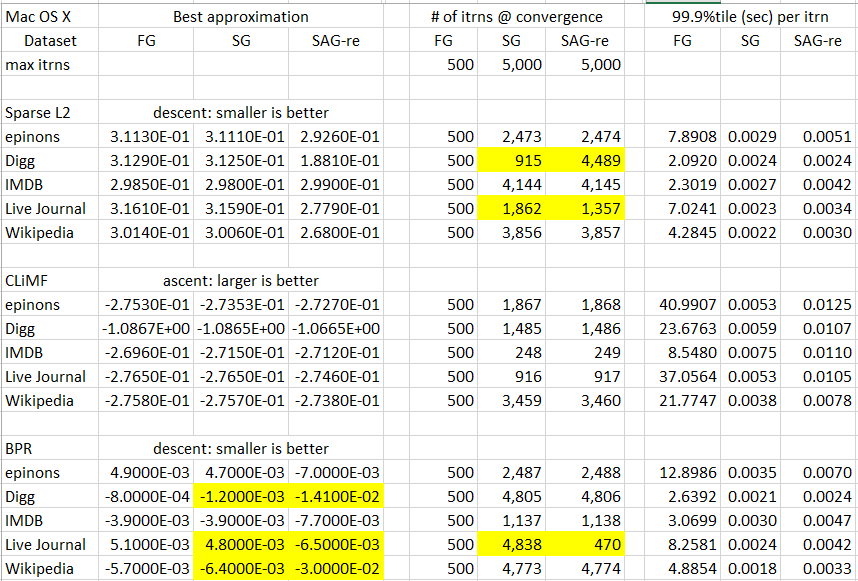
\includegraphics[width=6.1in, natwidth=851,natheight=574]{approx.png}}}
\caption[Optimization Quality among gradient methods]{Optimization Quality vs. Time among Full Deterministic Gradient (\emph{FG}), Stochastic Gradient (\emph{SG}), and \tool.}
\label{table:approx}
\end{figure*}


\header{Results and Discussion.}
The following is a legend to the metrics in figure \ref{table:approx}
\begin{sloppy}
\begin{compactenum}
\item \emph{Best Approximation}: 
the best quality optimization each gradient method achieved across different objective functions and various datasets.  
\item \emph{\# of itrns $@$ convergence}: 
the iteration at which each gradient achieved the best approximation.  
In full deterministic gradient (\emph{FG}), every incremental iteration gradient always yields a better quality optimization. 
In stochastic gradient (\emph{SG}), our observation confirms with theory that optimization quality would stay at a sub-optimum before the entire 5,000 iterations.
\tool behaves like stochastic gradient in most cases; the only different is that \tool consistently yielded a much better optimization than \emph{SG}.
\item \emph{99.9\%tile (sec) per itrn}
The 99.9 percentile time an iteration takes.  
When there are 5,000 iterations, we took the 5th longest iteration time.  
When there are 500 iterations, we took the 2nd longest iteration time.
Many literature in the systems area use 99.9 percentile time to guarantee a quality of service.  
In this case, we want to closely measure how much longer an iterationt \tool takes than \emph{SG}.
\end{compactenum}
\end{sloppy}

Stochastic gradient (\emph{SG}) yielded better quality optimizations in less than time full deterministic gradient (\emph{FG}).
The reason is that \emph{FG} takes 1,000 to 10,000 much longer to run an iteration than \emph{SG}.
\tool yielded much better quality optimizations than \emph{SG}; however \tool took up to 3 times longer to finish 5,000 iterations than \emph{SG}.
To enforce re-computation, we let \tool perform a full deterministic gradient at the first iteration.  
We observed that performing a full deterministic gradient at the first iteration sets \tool's optimization quality further apart from \emph{SG}'s.



\subsection{Follow-up Experiment}
\header{Methodology.}
To further study if \tool yields a better approximation in less time than \emph{SG}.  We ran a follow-up experiment.
We add up the total time \tool takes to reach convergence: 1 iteration of \emph{FG}, plus other iterations of re-computation.
Then, we transform this total time into the number of iterations for \emph{SG}, by dividing the total time by \emph{SG}'s unit iteration time. 
We measure whether \emph{SG} can yield a better optimization given the added number of iterations.  

\begin{figure*}
\centerline{\scalebox{1.00}{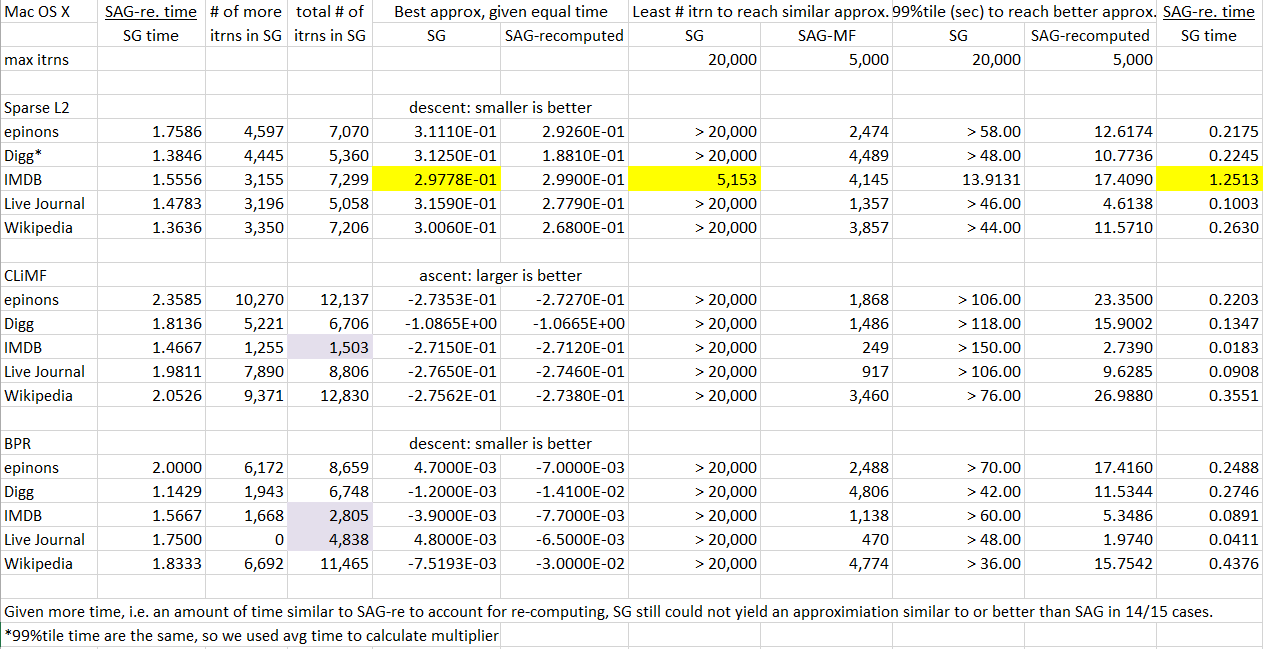
\includegraphics[width=8.2in, natwidth=1263,natheight=649]{followup.png}}}
\caption[Follow-up Experiment]{Follow-up experiment to determine if Stochastic Gradient (\emph{SG}) can yield a better approximation than \tool if \emph{SG} given more time in terms of more iterations.}
\label{table:followup}
\end{figure*}

\header{Results and Discussion.}
The following is a legend to the metrics in figure \ref{table:approx}
\begin{sloppy}
\begin{compactenum}
\item $\frac{\tool\:time}{\emph{SG}\:time}$: 
multiplier of how much longer an iteration would \tool takes than an iteration of \emph{SG}.  
An iteration of \tool takes up to 3 times as long as an iteration of \emph{SG}.
\item \emph{\# of more itrns in SG}: 
how many more bonus iterations we give to \emph{SG} so that we give \emph{SG} and \tool an equal amount of time to run their optimizations
\item \emph{total \# of itrns in SG}: 
total number of iterations \emph{SG} has we give \emph{SG} the bonus iterations
\item \emph{Best approx, given equal time}:
the best optimzation quality \emph{SG} and \tool achieve when both gradient methods have an equal amount of time to run optimization.
In most cases, optimization quality of \emph{SG} did not improve despite given more iterations and more time.
\item \emph{Least \# itrn to reach similar approx}:
We measure how much longer \emph{SG} takes to reach a quality of optimization similar to \tool.
However, even given a total of 20,000 iterations, \emph{SG} still yielded optimization quality worse than \tool.
\item \emph{99.9\%tile (sec) to reach better approx.}:
amount of time that \emph{SG} takes to reach a quality of optimization better than \tool.
\tool still outperformed \emph{SG} even \emph{SG} has 20,000 iterations, and \tool has only 5,000.
\item $\frac{\tool\:time}{\emph{SG}\:time}$: effective time to reach a similar quality of optimization;
this column shows \tool is at least 4 times faster than \emph{SG} to reach a similar quality of optimization.
\end{compactenum}
\end{sloppy}

A limitation in the follow-up experiment is the small number of non-zero entries in our sub-dataset.  
If there are more non-zero entries, than \emph{SG} would be given more iteraitons, because \tool performs an iteration of \emph{FG} at the start.
This is why we ran \emph{SG} for 20,000 iterations in total, and determine if 20,000 iterations of \emph{SG} can yield a better optimization than 5,000 iterations of \tool.
Our results indicate that in most cases, \emph{SG} would take more than 20,000 iterations to reach an optimization quality similar to \tool.
If we parallelize re-computation, then each iteration of \tool is faster and then we will give \emph{SG} less bonus iterations.  



\subsection{Space vs. Time}
\header{Methodology.}
We measure memory usage after the first iteration.

\begin{figure*}
\centerline{\scalebox{1.00}{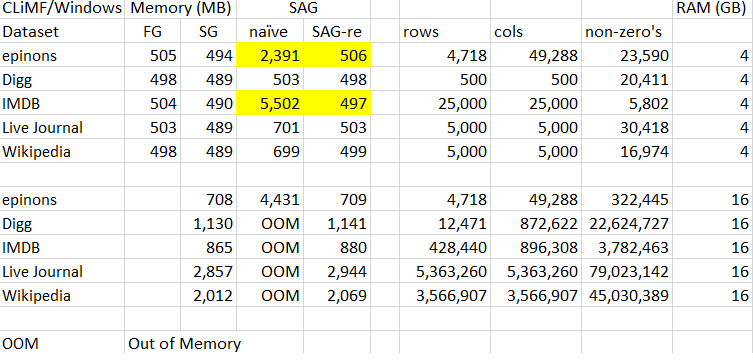
\includegraphics[width=6.0in, natwidth=753,natheight=362]{memory.png}}}
\caption[Memory usage after first iteration]{Memory usage between (\emph{FG}), Stochastic Gradient (\emph{SG}), and \tool after the first iteration of updating the CLiMF \cite{climf} objective function.}
\label{table:memory}
\end{figure*}

\header{Results and Discussion.}
When Matlab performs dynamic updates to sparse matrices, memory usage seems to depend more on the dimensionality of the sparse matrix 
(e.g. $(nRows*nCols)$-by-$nDims$) rather than $N$ the actual number of non-zero entries.

\tool also has an advantage at the low level of programming.
\tool stores $min(M,N)$ \emph{integers} as the predicted indices and does not update them.
In contrast, the na$\ddot{i}$ve approach of SAG must store $2*nMems*nDims$ \emph{floating points}, and the na$\ddot{i}$ve approach updates these floating points dynamically in runtime.

Therefore, in addition to providing dimensionality reduction, 
\tool decouples \emph{SAG}'s dependence on the low-level implementation of sparse matrices in the underlying programming language or execution environment.
Data Scientists do not need to spend time to find an efficient sparse-matrix implementation and integrate it into their code just to use \emph{SAG}.
